
\begin{section}{Geometry Generation}
\label{sec:workflow-geometries}


\begin{subsection}{Guiding Principles}


For any given monomer(s) of interest, the first step in the force field
development process is to choose a series of optimal dimer
configurations. This `optimal' set is highly dependent on the type of force field that
is being fit, and indeed the recommendations offered below are specific to the
\sapt-based force fields described in \cref{ch:isaff,ch:mastiff}.

\begin{figure}
\centering
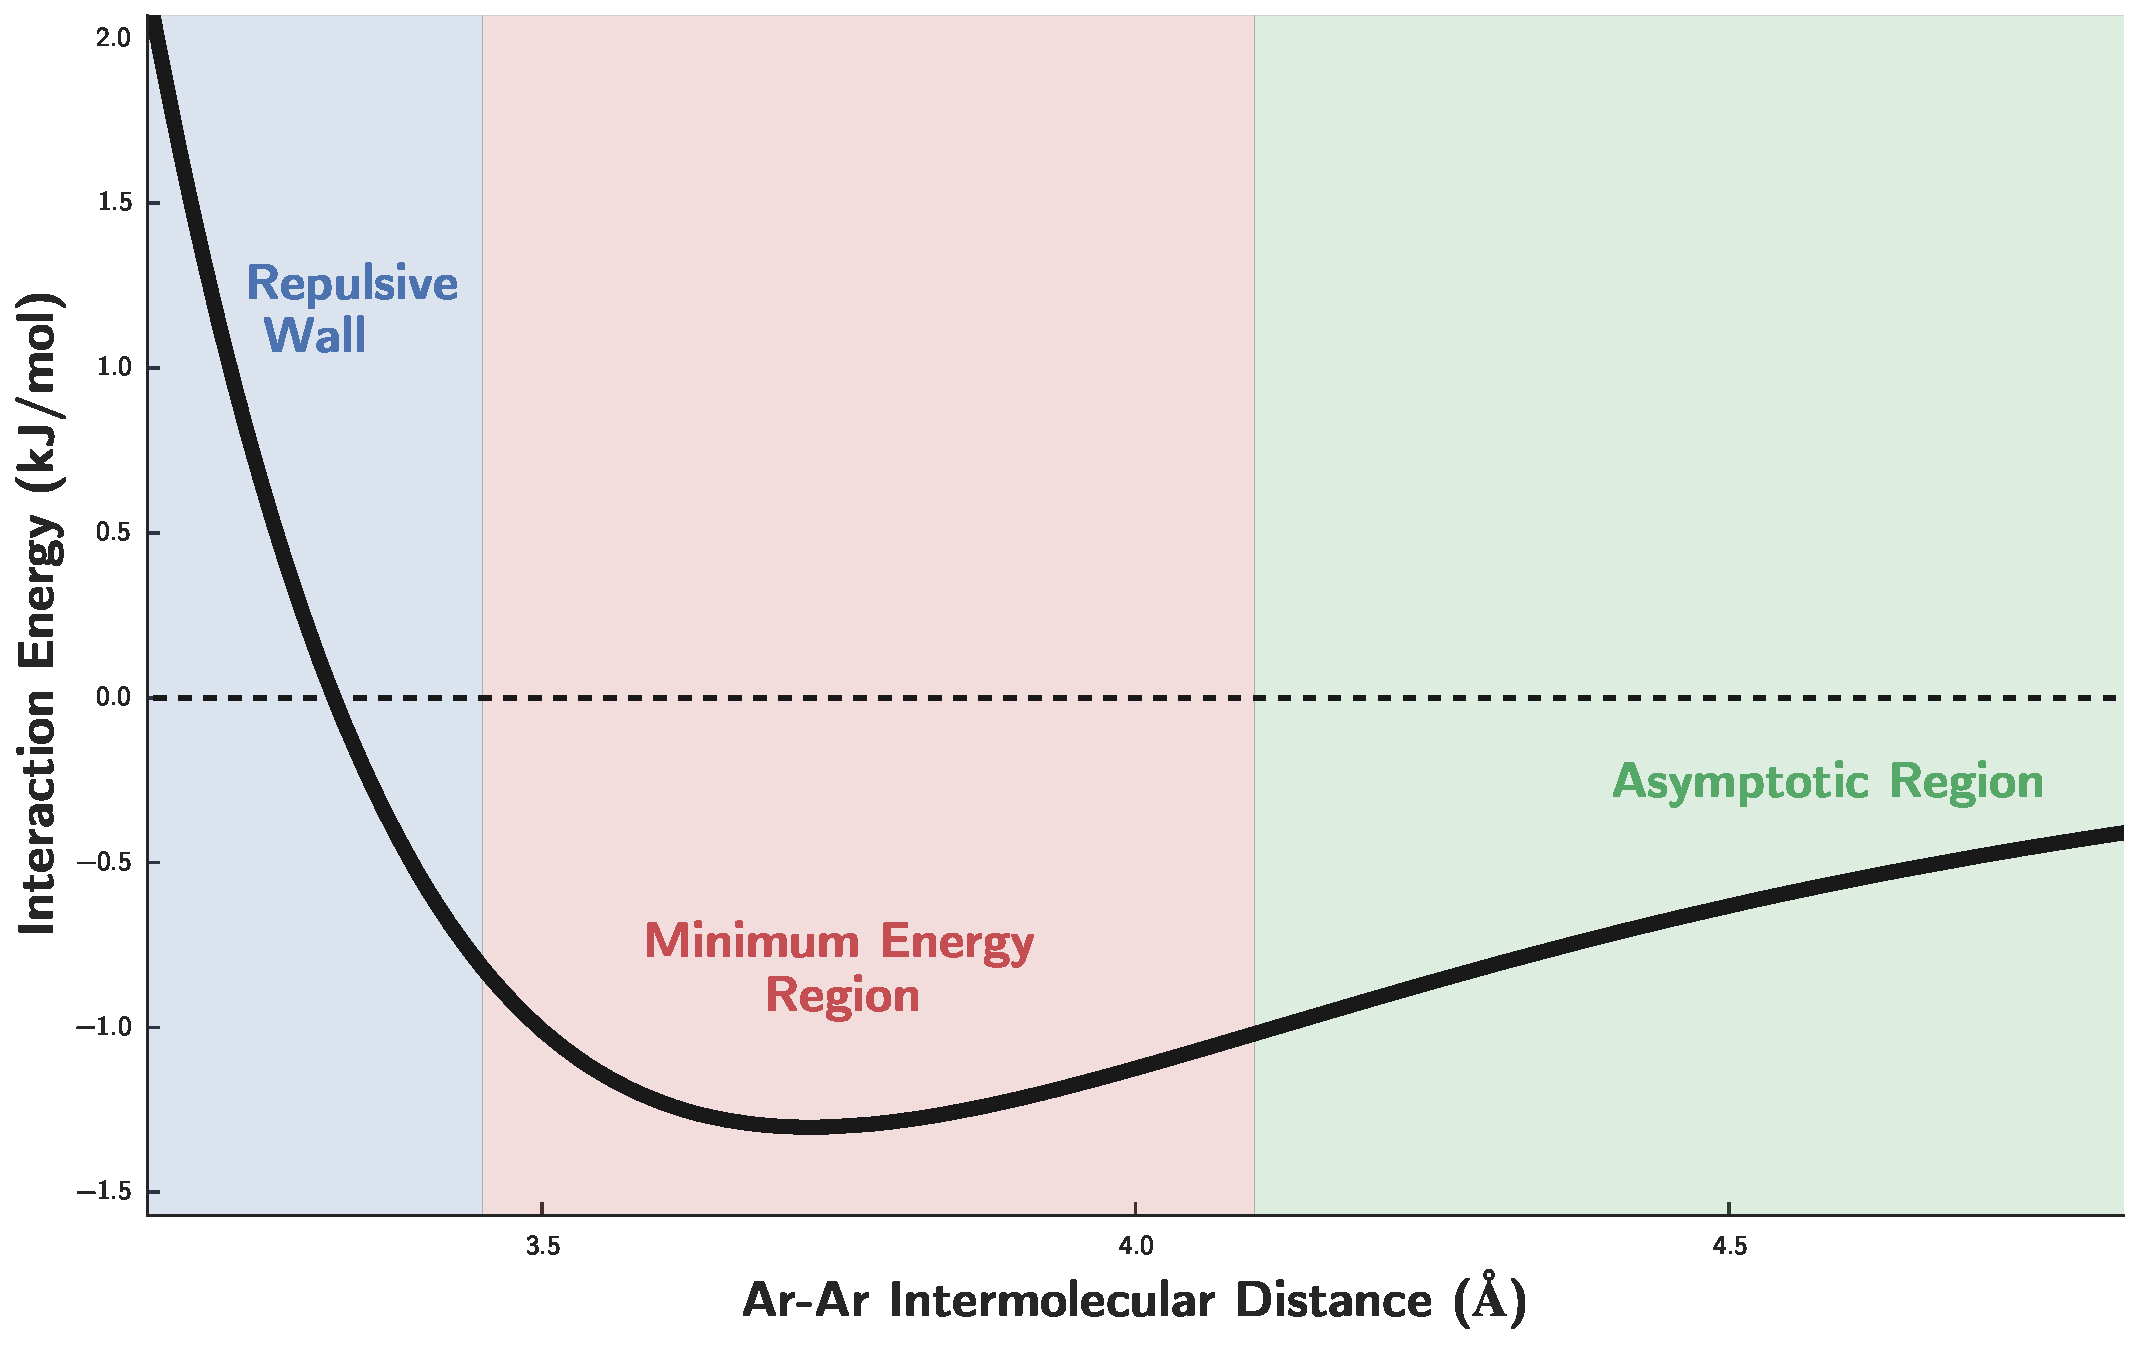
\includegraphics[width=1.0\textwidth]{workflow/generalized_pes.pdf}
\caption[Generalized form of a \pes showing the repulsive wall, minimum
energy, and asymptotic regions.]
        {Generalized form of a \pes showing the repulsive wall, minimum
energy, and asymptotic regions of the argon dimer. Cutoffs between the
different regions should be taken qualitatively.}
\label{fig:workflow-pes}
\end{figure}

In general, and as shown in \cref{fig:workflow-pes}, a given \pes will have (qualitatively) three different regions: a
repulsive wall, a minimum energy region, and an asymptotic region (which is
often attractive, but which may be repulsive due to unfavorable
electrostatic interactions). Due to the nature of the Boltzmann distribution, \emph{routine molecular simulation will most frequently
sample the minimum energy and asymptotic regions of the potential, making
these portions of the \pes the most important to model correctly}.
Nevertheless, and as discussed in \cref{sec:workflow-monomer_parameters}, the
asymptotic region of the \pes primarily depends on functionals forms whose
parameters are calculated from monomer properties, making 
the dimer-based fits described in \cref{ch:pointer} relatively insensitive to
inclusion of configurations in this %region.
region.\footnote{By contrast, other functional forms (e.g. Lennard-Jones) \emph{do}
have parameters that effect the asymptotic region, and for these force fields
it would be important to include this region in the parameterization process.}
%
By contrast, the fitted force field parameters largely determine the shape of
the repulsive wall and (to a lesser extent) the minimum energy regions, and so in practice we primarily
focus on including dimer configurations in these %regime.
%
regimes.\footnote{Historical note: For force field functional forms which
poorly model the repulsive wall (e.g. Lennard-Jones force fields or the \saptff
described in \cref{ch:isaff}), 
the force field fit quality is highly sensitive to the
relative representation of repulsive and attractive dimer configurations.
(Including both too few or too many repulsive configurations can be
problematic). Only with the advent of \isaffold and \mastiff has the
fit quality become strictly improved by including repulsive configurations.}
%
In other words, and based on a combination of importance in molecular
simulation and fit sensitivity to the specific parameters which we are directly
optimizing, \emph{the repulsive wall and especially the minimum energy regions are the
most important to effectively sample in order to achieve good force field fits}.

As described below, a standard procedure for the properly sampling across the
\pes has been established for the \isaffold
and \mastiff force fields. Only when fitting different functional forms will
the user need to reconsider the relative sampling of dimer configurations.

\end{subsection}
\begin{subsection}{Theory}

Assuming rigid monomer geometries, a dimer configuration can be completely
determined (without loss of generalization) by fixing the first monomer at the
origin and by placing the second monomer according to the following six variables: $r$, $\theta$, and $\phi$ determine the position
of center of mass of the second monomer, and the three-dimensional variable $\Omega$ determines the relative
orientation of the monomer about its center of mass. In practice, $\Omega$ is
most easily described by a quaternion approach, see \citen{Guibas1992}.

For both the \isaffold and \mastiff fits, dimer configurations are sampled
psuedo-randomly using Shoemake's algorithm\cite{Shoemake1992} (which ensures even sampling across
the center of mass orientation) subject to some exclusion criteria.
In particular, and in order to achieve representative sampling of the
repulsive wall and minimum energy regions, the following dimer configurations
are excluded from sampling:
\begin{enumerate}
\item Configurations with any atom-atom contact distance 
$r_{ij} \le 0.8\times(r^{\text{vdw}}_i + r^{\text{vdw}}_j)$, where $r_{ij}$ is the
contact distance and $r^{\text{vdw}}$ is the tabulated van der Waals radius
for a given element
\item Configurations with all atom-atom contact distance 
$r_{ij} \ge 1.3\times(r^{\text{vdw}}_i + r^{\text{vdw}}_j)$
\end{enumerate}


\end{subsection}
\begin{subsection}{Practicals}

In practice, generation of the dimer configurations is fairly straightforward.
The required input files -- \verb|dimer_info.dat|,
\verb|generate_grid_settings.inp|, and \verb|<mona>_<monb>.inp| --
are
listed  in
\cref{lst:workflow-generate_geometries,lst:workflow-dimer_info,lst:workflow-dimer_geom}
and using the pyridine dimer as an example.
Each input file may need to be modified for the dimer under consideration, and
comments within each input file explain any necessary system-specific changes.



Once these input files have been modified, the geometry generation process can
be carried out very simply from the main force field fitting directory by
executing the command

\begin{lstlisting}
./scripts/make_geometries.sh
\end{lstlisting}

\end{subsection}


\end{section}
